% Source PDF page 161 (printed p. 147)
\begin{figure}[htbp]
\centering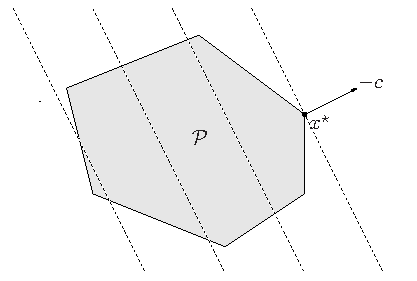
\includegraphics[width=.50\textwidth]{figures/ch04-04.pdf}
\caption*{图4.4\quad LP的几何解释。阴影部分为多面体可行集 $\mathcal P$。目标 $c^\T x$ 线性，所以其等高线是垂直于 $c$ 的超平面（虚线）。点 $x^\star$ 最优，它是 $\mathcal P$ 中沿 $-c$ 方向最远的点。}
\end{figure}
\begin{equation}
\begin{array}{ll}\text{最小化}&c^\T x\\\text{约束为}&Ax=b,\\&x\succeq0.\end{array}\tag{4.28}
\end{equation}
若LP没有等式约束，称为不等式形式LP，通常写为
\begin{equation}
\begin{array}{ll}\text{最小化}&c^\T x\\\text{约束为}&Ax\preceq b.\end{array}\tag{4.29}
\end{equation}

\subsubsection*{将LP转化为标准形式}
有时将一般LP（4.27）转化为标准形式（4.28）很有用，例如为了使用求解标准形式LP的算法。第一步为不等式引入松弛变量 $s_i$，得到
\[
\begin{array}{ll}\text{最小化}&c^\T x+d\\\text{约束为}&Gx+s=h,\\&Ax=b,\\&s\succeq0.\end{array}
\]
第二步将变量 $x$ 表示为两个非负变量 $x^+$、$x^-$ 的差，即 $x=x^+-x^-$，$x^+,x^-\succeq0$，得到
\[
\begin{array}{ll}
\text{最小化}&c^\T x^+-c^\T x^-+d\\
\text{约束为}&Gx^+-Gx^-+s=h,\\
&Ax^+-Ax^-=b,\\
&x^+\succeq0,\quad x^-\succeq0,\quad s\succeq0.
\end{array}
\]

% Source PDF page 162 (printed p. 148)
这是以 $x^+,x^-,s$ 为变量的标准形式LP。（此问题与原问题（4.27）的等价性见习题4.10。）

这些问题变换技巧，加上后面的例子和习题中会介绍的许多其他技巧，可以将大量问题表述为线性规划。用语上常作一定放宽：即使一个问题本身不具有（4.27）的形式，只要能表述为LP，通常也将其称为LP。

\subsection{例子}
LP出现在大量领域和应用中，下面给出几个典型例子。

\subsubsection*{膳食问题}
健康膳食需要包含 $m$ 种不同营养素，其数量至少分别为 $b_1,\ldots,b_m$。可从 $n$ 种食物中选择非负数量 $x_1,\ldots,x_n$，组成这种膳食。每单位食物 $j$ 含有数量为 $a_{ij}$ 的营养素 $i$，成本为 $c_j$。我们要确定满足营养要求的最便宜膳食。此问题可表述为LP
\[
\begin{array}{ll}\text{最小化}&c^\T x\\\text{约束为}&Ax\succeq b,\\&x\succeq0.\end{array}
\]
这个问题的若干变体也可以表述为LP。例如，可要求某种营养素的数量精确等于指定值，从而得到线性等式约束；也可在上述下界之外，再对营养素的数量施加上界。

\subsubsection*{多面体的Chebyshev中心}
考虑在由线性不等式描述的多面体
\[
\mathcal P=\{x\in\R^n\mid a_i^\T x\le b_i,\ i=1,\ldots,m\}
\]
中寻找最大欧氏球的问题。（最优球的中心称为多面体的Chebyshev中心；它是多面体内部最深的点，即离边界最远的点，见§8.5.1。）将球表示为
\[
\mathcal B=\{x_c+u\mid\norm{u}_2\le r\}.
\]
问题的变量为球心 $x_c\in\R^n$ 和半径 $r$，目标是在 $\mathcal B\subseteq\mathcal P$ 的约束下最大化 $r$。

先考虑较简单的约束：$\mathcal B$ 位于一个半空间 $a_i^\T x\le b_i$ 中，即
\begin{equation}
\norm{u}_2\le r\quad\Longrightarrow\quad a_i^\T(x_c+u)\le b_i.\tag{4.30}
\end{equation}
由于
\[
\sup\{a_i^\T u\mid\norm{u}_2\le r\}=r\norm{a_i}_2,
\]

% Source PDF page 163 (printed p. 149)
可以将（4.30）写为
\begin{equation}
a_i^\T x_c+r\norm{a_i}_2\le b_i,\tag{4.31}
\end{equation}
它是关于 $x_c,r$ 的线性不等式。换言之，球包含于不等式 $a_i^\T x\le b_i$ 所确定半空间的约束，可以写成线性不等式。

所以 $\mathcal B\subseteq\mathcal P$ 当且仅当（4.31）对所有 $i=1,\ldots,m$ 成立。因此，求解LP
\[
\begin{array}{ll}\text{最大化}&r\\\text{约束为}&a_i^\T x_c+r\norm{a_i}_2\le b_i,\quad i=1,\ldots,m\end{array}
\]
即可确定Chebyshev中心，变量为 $r,x_c$。（更多关于Chebyshev中心的内容见§8.5.1。）

\subsubsection*{动态活动规划}
考虑在 $N$ 个时期内，为 $n$ 项活动或经济部门选择、规划活动水平的问题。以 $x_j(t)\ge0$（$t=1,\ldots,N$）表示部门 $j$ 在第 $t$ 期的活动水平。活动按其水平成比例地消耗和生产产品或物品。每单位活动 $j$ 生产的物品 $i$ 的数量为 $a_{ij}$；类似地，每单位活动 $j$ 消耗的物品 $i$ 的数量为 $b_{ij}$。第 $t$ 期的总产出为 $Ax(t)\in\R^m$，总消耗为 $Bx(t)\in\R^m$。（虽然称这些产品为“物品”，它们也可以包括污染物等不需要的产物。）

每期消耗的物品不能超过前一期生产的物品，即要求 $Bx(t+1)\preceq Ax(t)$（$t=1,\ldots,N$）。给定初始物品向量 $g_0\in\R^m$，它限制第一期活动水平：$Bx(1)\preceq g_0$。未被活动消耗的剩余物品向量为
\[
\begin{aligned}
s(0)&=g_0-Bx(1),\\
s(t)&=Ax(t)-Bx(t+1),\quad t=1,\ldots,N-1,\\
s(N)&=Ax(N).
\end{aligned}
\]
目标是最大化剩余物品的折现总价值：
\[
c^\T s(0)+\gamma c^\T s(1)+\cdots+\gamma^N c^\T s(N),
\]
其中 $c\in\R^m$ 给出物品的价值，$\gamma>0$ 为折现因子。（若第 $i$ 种产品是不需要的，例如污染物，则 $c_i$ 为负数，此时 $|c_i|$ 为单位处置成本。）

综上，得到LP
\[
\begin{array}{ll}
\text{最大化}&c^\T s(0)+\gamma c^\T s(1)+\cdots+\gamma^N c^\T s(N)\\
\text{约束为}&x(t)\succeq0,\quad t=1,\ldots,N,\\
&s(t)\succeq0,\quad t=0,\ldots,N,\\
&s(0)=g_0-Bx(1),\\
&s(t)=Ax(t)-Bx(t+1),\quad t=1,\ldots,N-1,\\
&s(N)=Ax(N),
\end{array}
\]
变量为 $x(1),\ldots,x(N),s(0),\ldots,s(N)$。这是标准形式LP，变量 $s(t)$ 是约束 $Bx(t+1)\preceq Ax(t)$ 对应的松弛变量。

% Source PDF page 164 (printed p. 150)
\subsubsection*{Chebyshev不等式}
考虑离散随机变量 $x$ 在有 $n$ 个元素的集合 $\{u_1,\ldots,u_n\}\subseteq\R$ 上的概率分布。以向量 $p\in\R^n$ 描述 $x$ 的分布，其中
\[
p_i=\Prob(x=u_i),
\]
因此 $p\succeq0$、$\one^\T p=1$。反过来，若 $p$ 满足这两个条件，它就定义了 $x$ 的一个概率分布。假设 $u_i$ 已知且固定，但分布 $p$ 未知。

对 $x$ 的任意函数 $f$，
\[
\E f=\sum_{i=1}^n p_if(u_i)
\]
是 $p$ 的线性函数。对 $\R$ 的任意子集 $S$，
\[
\Prob(x\in S)=\sum_{u_i\in S}p_i
\]
也是 $p$ 的线性函数。

虽然不知道 $p$，但给定如下先验知识：知道 $x$ 的某些函数的期望，以及某些 $\R$ 的子集的概率的上下界。这些先验知识可表示为关于 $p$ 的线性不等式约束
\[
\alpha_i\le a_i^\T p\le\beta_i,\quad i=1,\ldots,m.
\]
问题是为 $\E f_0(x)=a_0^\T p$ 给出上下界，其中 $f_0$ 是 $x$ 的某个函数。

为求下界，解以 $p$ 为变量的LP
\[
\begin{array}{ll}\text{最小化}&a_0^\T p\\\text{约束为}&p\succeq0,\quad\one^\T p=1,\\&\alpha_i\le a_i^\T p\le\beta_i,\quad i=1,\ldots,m.\end{array}
\]
这个LP的最优值给出了与先验信息相容的所有分布中 $\E f_0(X)$ 的最小可能值。而且此界是紧的：最优解给出一个与先验信息相容且达到下界的分布。类似地，在相同约束下最大化 $a_0^\T p$，可得最佳上界。（§7.4.1将更详细地讨论Chebyshev不等式。）

\subsubsection*{分段线性函数最小化}
考虑无约束最小化分段线性凸函数
\[
f(x)=\max_{i=1,\ldots,m}(a_i^\T x+b_i)
\]
的问题。先取上图形式
\[
\begin{array}{ll}\text{最小化}&t\\\text{约束为}&\max_{i=1,\ldots,m}(a_i^\T x+b_i)\le t,\end{array}
\]
再将不等式改写为 $m$ 个单独的不等式，即可变为等价LP：

% Source PDF page 165 (printed p. 151)
\[
\begin{array}{ll}\text{最小化}&t\\\text{约束为}&a_i^\T x+b_i\le t,\quad i=1,\ldots,m.\end{array}
\]
这是以 $x,t$ 为变量的不等式形式LP。

\subsection{线性分式规划}
在多面体上最小化两个仿射函数之比的问题，称为线性分式规划：
\begin{equation}
\begin{array}{ll}\text{最小化}&f_0(x)\\\text{约束为}&Gx\preceq h,\\&Ax=b,\end{array}\tag{4.32}
\end{equation}
其中目标为
\[
f_0(x)=\frac{c^\T x+d}{e^\T x+f},\qquad\dom f_0=\{x\mid e^\T x+f>0\}.
\]
目标函数拟凸，实际上是拟线性的，因此线性分式规划是拟凸优化问题。

\subsubsection*{转化为线性规划}
若可行集
\[
\{x\mid Gx\preceq h,\ Ax=b,\ e^\T x+f>0\}
\]
非空，线性分式规划（4.32）可转化为以 $y,z$ 为变量的等价LP
\begin{equation}
\begin{array}{ll}
\text{最小化}&c^\T y+dz\\
\text{约束为}&Gy-hz\preceq0,\\
&Ay-bz=0,\\
&e^\T y+fz=1,\\
&z\ge0.
\end{array}\tag{4.33}
\end{equation}
为说明等价性，先注意，若 $x$ 对（4.32）可行，则
\[
y=\frac{x}{e^\T x+f},\qquad z=\frac{1}{e^\T x+f}
\]
对（4.33）可行，且目标值相同，即 $c^\T y+dz=f_0(x)$。所以（4.32）的最优值大于等于（4.33）的最优值。

反过来，若 $(y,z)$ 对（4.33）可行且 $z\ne0$，则 $x=y/z$ 对（4.32）可行，且目标值相同：$f_0(x)=c^\T y+dz$。若 $(y,z)$ 对（4.33）可行且 $z=0$，另有 $x_0$ 对（4.32）可行，则对所有 $t\ge0$，$x=x_0+ty$ 对（4.32）可行。而且 $\lim_{t\to\infty}f_0(x_0+ty)=c^\T y+dz$，所以可找到（4.32）的可行点，使目标值任意接近 $(y,z)$ 的目标值。由此可知，（4.32）的最优值小于等于（4.33）的最优值。

% Source PDF page 166 (printed p. 152)
\subsubsection*{广义线性分式规划}
线性分式规划（4.32）的一种推广为广义线性分式规划，其中
\[
f_0(x)=\max_{i=1,\ldots,r}\frac{c_i^\T x+d_i}{e_i^\T x+f_i},\qquad
\dom f_0=\{x\mid e_i^\T x+f_i>0,\ i=1,\ldots,r\}.
\]
目标为 $r$ 个拟凸函数的逐点最大值，因而拟凸，所以此问题为拟凸问题。当 $r=1$ 时，它退化为普通线性分式规划。

\begin{origexample}{4.7}
\textbf{Von Neumann增长问题。}考虑有 $n$ 个部门的经济系统，当前期活动水平为 $x_i>0$，下一期为 $x_i^+>0$。（此处只考虑一个时期。）活动既消耗也生产 $m$ 种物品：活动水平 $x$ 消耗物品 $Bx\in\R^m$，生产物品 $Ax$。下一期消耗不能超过当前期产出，即 $Bx^+\preceq Ax$。部门 $i$ 在此期间的增长率为 $x_i^+/x_i$。

Von Neumann增长问题是寻找活动水平向量 $x$，使全部部门中的最小增长率最大。此问题可表示为广义线性分式问题
\[
\begin{array}{ll}\text{最大化}&\min_{i=1,\ldots,n}x_i^+/x_i\\\text{约束为}&x^+\succeq0,\\&Bx^+\preceq Ax,\end{array}
\]
定义域为 $\{(x,x^+)\mid x\succ0\}$。注意，此问题关于 $x,x^+$ 齐次，因此可用显式约束 $x\succeq\one$ 替换隐式约束 $x\succ0$。
\end{origexample}

\section{二次优化问题}
若凸优化问题（4.15）的目标为凸二次函数，约束函数为仿射函数，就称为二次规划（QP）。二次规划可表示为
\begin{equation}
\begin{array}{ll}\text{最小化}&(1/2)x^\T Px+q^\T x+r\\\text{约束为}&Gx\preceq h,\\&Ax=b,\end{array}\tag{4.34}
\end{equation}
其中 $P\in\mathbf S_+^n$、$G\in\R^{m\times n}$、$A\in\R^{p\times n}$。二次规划是在多面体上最小化凸二次函数，如图4.5。

若（4.15）的目标和不等式约束函数均为凸二次函数，如
\begin{equation}
\begin{array}{ll}
\text{最小化}&(1/2)x^\T P_0x+q_0^\T x+r_0\\
\text{约束为}&(1/2)x^\T P_ix+q_i^\T x+r_i\le0,\quad i=1,\ldots,m,\\
&Ax=b,
\end{array}\tag{4.35}
\end{equation}

% Source PDF page 167 (printed p. 153)
\begin{figure}[htbp]
\centering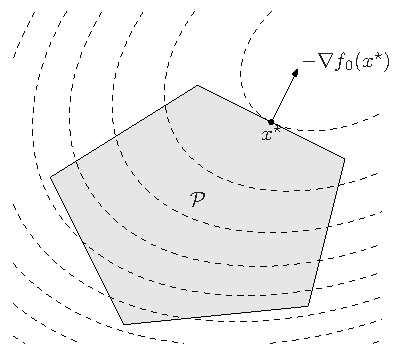
\includegraphics[width=.50\textwidth]{figures/ch04-05.pdf}
\caption*{图4.5\quad QP的几何示意。阴影部分为多面体可行集 $\mathcal P$，虚线为凸二次目标函数的等高线。点 $x^\star$ 最优。}
\end{figure}
其中 $P_i\in\mathbf S_+^n$（$i=0,1,\ldots,m$），就称为二次约束二次规划（QCQP）。QCQP在椭球的交构成的可行域上最小化凸二次函数，这里椭球情形对应 $P_i\succ0$。

二次规划包含线性规划这一特例，只需在（4.34）中取 $P=0$。二次约束二次规划包含二次规划，因而也包含线性规划这一特例，只需在（4.35）中对 $i=1,\ldots,m$ 取 $P_i=0$。

\subsection{例子}
\subsubsection*{最小二乘与回归}
最小化凸二次函数
\[
\norm{Ax-b}_2^2=x^\T A^\T Ax-2b^\T Ax+b^\T b
\]
的问题是无约束QP。它出现在许多领域，有许多名称，如回归分析或最小二乘逼近。这个问题足够简单，具有熟知的解析解 $x=A^\dagger b$，其中 $A^\dagger$ 为 $A$ 的伪逆，见§A.5.4。

加入线性不等式约束后，称为约束回归或约束最小二乘，此时不再有简单的解析解。例如，考虑对变量施加上下界的回归问题
\[
\begin{array}{ll}\text{最小化}&\norm{Ax-b}_2^2\\\text{约束为}&l_i\le x_i\le u_i,\quad i=1,\ldots,n,\end{array}
\]

% Source PDF page 168 (printed p. 154)
这是QP。（第6章和第7章将更深入研究最小二乘和回归问题。）

\subsubsection*{多面体之间的距离}
$\R^n$ 中两个多面体 $\mathcal P_1=\{x\mid A_1x\preceq b_1\}$ 与 $\mathcal P_2=\{x\mid A_2x\preceq b_2\}$ 的欧氏距离定义为
\[
\dist(\mathcal P_1,\mathcal P_2)=\inf\{\norm{x_1-x_2}_2\mid x_1\in\mathcal P_1,\ x_2\in\mathcal P_2\}.
\]
若两个多面体相交，距离为零。

为求 $\mathcal P_1$ 与 $\mathcal P_2$ 的距离，可解以 $x_1,x_2\in\R^n$ 为变量的QP
\[
\begin{array}{ll}\text{最小化}&\norm{x_1-x_2}_2^2\\\text{约束为}&A_1x_1\preceq b_1,\quad A_2x_2\preceq b_2.\end{array}
\]
当且仅当至少一个多面体为空时，此问题不可行。当且仅当两个多面体相交时，最优值为零，此时最优 $x_1,x_2$ 相等，并位于交集 $\mathcal P_1\cap\mathcal P_2$ 中。否则，最优 $x_1,x_2$ 分别是两个多面体中彼此距离最近的点。（第8章将进一步研究涉及距离的几何问题。）

\subsubsection*{方差的界}
再次考虑第150页Chebyshev不等式的例子，变量为向量 $p\in\R^n$ 给出的未知概率分布，已知它的一些先验信息。随机变量 $f(x)$ 的方差为
\[
\E f^2-(\E f)^2=\sum_{i=1}^n f_i^2p_i-\left(\sum_{i=1}^n f_ip_i\right)^2,
\]
其中 $f_i=f(u_i)$，它是 $p$ 的凹二次函数。

因此，在给定先验信息约束下最大化 $f(x)$ 的方差，可以求解QP
\[
\begin{array}{ll}
\text{最大化}&\displaystyle\sum_{i=1}^n f_i^2p_i-\left(\sum_{i=1}^n f_ip_i\right)^2\\
\text{约束为}&p\succeq0,\quad\one^\T p=1,\\
&\alpha_i\le a_i^\T p\le\beta_i,\quad i=1,\ldots,m.
\end{array}
\]
最优值是在全部与先验信息相容的分布中 $f(x)$ 的最大可能方差；最优 $p$ 给出达到该最大方差的分布。

\subsubsection*{随机成本的线性规划}
考虑以 $x\in\R^n$ 为变量的LP
\[
\begin{array}{ll}\text{最小化}&c^\T x\\\text{约束为}&Gx\preceq h,\\&Ax=b.\end{array}
\]

% Source PDF page 169 (printed p. 155)
假设成本向量 $c\in\R^n$ 为随机变量，均值为 $\bar c$，协方差为 $\E(c-\bar c)(c-\bar c)^\T=\Sigma$。（为简单起见，假设其余问题参数均为确定量。）给定 $x\in\R^n$，成本 $c^\T x$ 是标量随机变量，其均值为 $\E c^\T x=\bar c^\T x$，方差为
\[
\operatorname{var}(c^\T x)=\E(c^\T x-\E c^\T x)^2=x^\T\Sigma x.
\]
通常需要在较小的期望成本与较小的成本方差之间取舍。考虑方差的一种方式，是最小化成本期望和方差的线性组合
\[
\E c^\T x+\gamma\operatorname{var}(c^\T x),
\]
称为风险敏感成本。参数 $\gamma\ge0$ 称为风险厌恶参数，因为它规定成本方差与期望的相对价值。（$\gamma>0$ 时，我们愿意接受期望成本增加，以换取足够大的成本方差下降。）

最小化风险敏感成本，就是求解QP
\[
\begin{array}{ll}\text{最小化}&\bar c^\T x+\gamma x^\T\Sigma x\\\text{约束为}&Gx\preceq h,\\&Ax=b.\end{array}
\]

\subsubsection*{Markowitz投资组合优化}
考虑在一段时期内持有 $n$ 种资产或股票的经典投资组合问题。以 $x_i$ 表示整个时期持有的资产 $i$ 的数量，按期初价格以美元计。资产 $i$ 的普通多头头寸对应 $x_i>0$；空头头寸，即期末购买该资产的义务，对应 $x_i<0$。以 $p_i$ 表示该时期资产 $i$ 的相对价格变化，即价格变化除以期初价格。整个投资组合的收益为 $r=p^\T x$，单位为美元。优化变量为投资组合向量 $x\in\R^n$。

可以考虑多种投资组合约束。最简单的是 $x_i\ge0$（没有空头头寸）和 $\one^\T x=B$（总投资预算为 $B$，通常取一）。

采用价格变化的随机模型：$p\in\R^n$ 为随机向量，均值 $\bar p$ 和协方差 $\Sigma$ 已知。因此，对投资组合 $x\in\R^n$，收益 $r$ 为标量随机变量，均值为 $\bar p^\T x$，方差为 $x^\T\Sigma x$。选择投资组合 $x$ 就涉及收益均值与方差的取舍。

Markowitz提出的经典投资组合优化问题是QP
\[
\begin{array}{ll}\text{最小化}&x^\T\Sigma x\\\text{约束为}&\bar p^\T x\ge r_{\min},\\&\one^\T x=1,\quad x\succeq0,\end{array}
\]
其中投资组合 $x$ 为变量。这里寻找使收益方差最小的投资组合，收益方差与组合风险相关，同时要求达到可接受的最低平均收益 $r_{\min}$，并满足预算和禁止卖空约束。

% Source PDF page 170 (printed p. 156)
这个问题有许多推广。例如，一个标准推广是允许空头头寸，即允许 $x_i<0$。为此引入变量 $x^{\mathrm{long}},x^{\mathrm{short}}$，满足
\[
x^{\mathrm{long}}\succeq0,\quad x^{\mathrm{short}}\succeq0,\quad
x=x^{\mathrm{long}}-x^{\mathrm{short}},\quad
\one^\T x^{\mathrm{short}}\le\eta\one^\T x^{\mathrm{long}}.
\]
最后一个约束将期初总空头头寸限制为期初总多头头寸的某个比例 $\eta$。

另一个推广是在投资组合优化中计入线性交易成本。从给定初始投资组合 $x^{\mathrm{init}}$ 出发，通过买卖资产得到投资组合 $x$，然后按前述方式持有一个时期。买卖收取与交易数量成比例的交易费。为处理这一点，引入变量 $u^{\mathrm{buy}},u^{\mathrm{sell}}$，分别表示持有期开始前买入、卖出的各项资产数量，约束为
\[
x=x^{\mathrm{init}}+u^{\mathrm{buy}}-u^{\mathrm{sell}},\qquad
u^{\mathrm{buy}}\succeq0,\quad u^{\mathrm{sell}}\succeq0.
\]
用初始买卖包括交易费的净现金流为零，替换简单预算约束 $\one^\T x=1$：
\[
(1-f^{\mathrm{sell}})\one^\T u^{\mathrm{sell}}
=(1+f^{\mathrm{buy}})\one^\T u^{\mathrm{buy}}.
\]
左侧是卖出资产的总收入减去卖出交易费，右侧是买入资产包括交易费的总成本。常数 $f^{\mathrm{buy}}\ge0$、$f^{\mathrm{sell}}\ge0$ 分别为买入和卖出的费率，为简单起见，假设所有资产费率相同。

在最低平均收益、预算及交易约束下，最小化收益方差，是以 $x,u^{\mathrm{buy}},u^{\mathrm{sell}}$ 为变量的QP。

\subsection{二阶锥规划}
与二次规划密切相关的一类问题是二阶锥规划（SOCP）：
\begin{equation}
\begin{array}{ll}
\text{最小化}&f^\T x\\
\text{约束为}&\norm{A_ix+b_i}_2\le c_i^\T x+d_i,\quad i=1,\ldots,m,\\
&Fx=g,
\end{array}\tag{4.36}
\end{equation}
其中优化变量为 $x\in\R^n$，$A_i\in\R^{n_i\times n}$，$F\in\R^{p\times n}$。形如
\[
\norm{Ax+b}_2\le c^\T x+d,
\]
其中 $A\in\R^{k\times n}$，的约束称为二阶锥约束，因为它等价于要求仿射函数 $(Ax+b,c^\T x+d)$ 位于 $\R^{k+1}$ 的二阶锥中。

当 $c_i=0$（$i=1,\ldots,m$）时，SOCP（4.36）等价于QCQP，将各个约束平方即可得到。类似地，若 $A_i=0$（$i=1,\ldots,m$），则（4.36）退化为一般LP。不过，二阶锥规划比QCQP更加一般，当然也比LP更加一般。
